\textcolor{black}{\section{Resultados y Análisis}}

\noindent En la Figura \ref{Graf1} se puede observar los espectros de cada uno de los LEDs; se tomó como la longitud de onda $\lambda$ el valor máximo registrado en el espectro, y como es una distribución, se tomó como barra de incertidumbre el ancho del espectro medido desde la mitad de la altura máxima.

Entonces, con estos datos se utilizó la Ecuación \ref{eq:frec} para obtener las frecuencias de cada uno. La Figura $\ref{Graf2}$ muestra la gráfica de $\nu \text{ vs. } V_{U}$, en donde se realizó una regresión lineal omitiendo la medición más dispersa.

\begin{figure*}
	\centering
	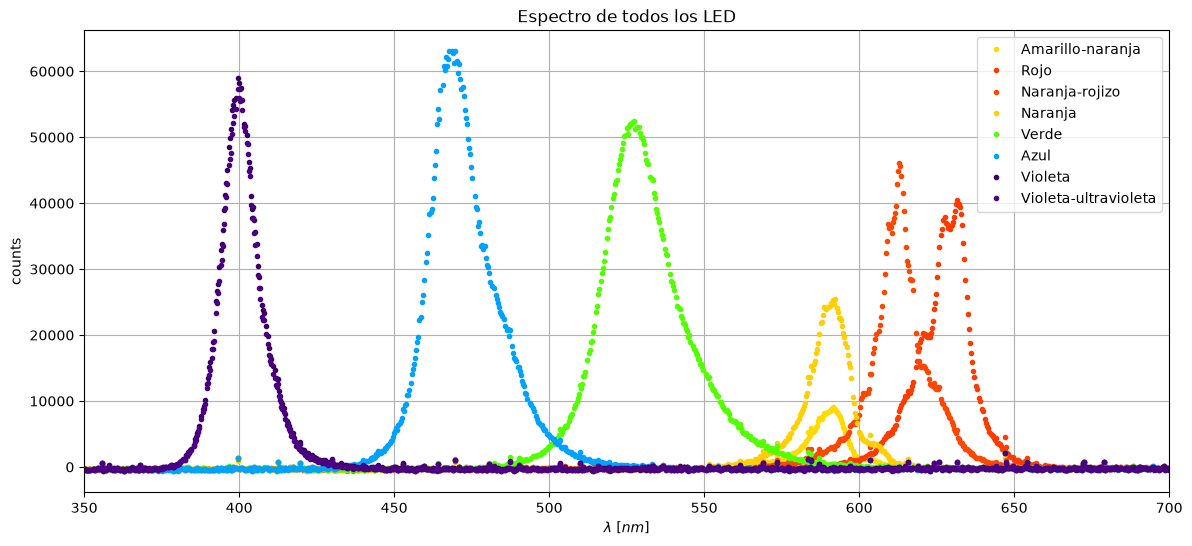
\includegraphics[scale=0.5]{figs/Graf1.png}
	\caption{Gráfica de los espectros de los 8 LEDs con el color asignado a la longitud máxima registrada de cada una.}
	\label{Graf1}
\end{figure*}

\begin{figure}[H]
	\centering
	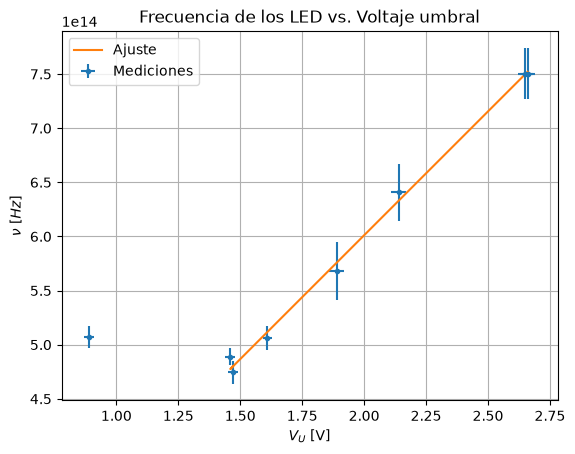
\includegraphics[scale=0.5]{figs/Graf2.png}
	\caption{Gráfica de las frecuencias de cada LED con el las mediciones del voltaje ánodo-cátodo (diodo). Se tiene una $R^2 = 0.99633$.}
	\label{Graf2}
\end{figure}

Con esta regresión se obtuvo, al invertir la pendiente, un valor de
\begin{equation}\label{eq:resultado_nuestro}
	\frac{1}{m} = \frac{h}{e} = 4.370998e-15
\end{equation}
en unidades del SI.